\section{Nombre: Etalagmitas}\label{obs.rocas}
	\subsection{Descripción}
	Tres estalagmitas de tamaño mediano, se ubican sobre el techo de cuevas. Cuando el jugador pasa por debajo de ellas caen. Al hacer contacto con el jugador le reducen la cantidad de vida.
	\subsection{Esquema}
	Ver figura \ref{fig:rocas}.
	\begin{figure}
		\centering
		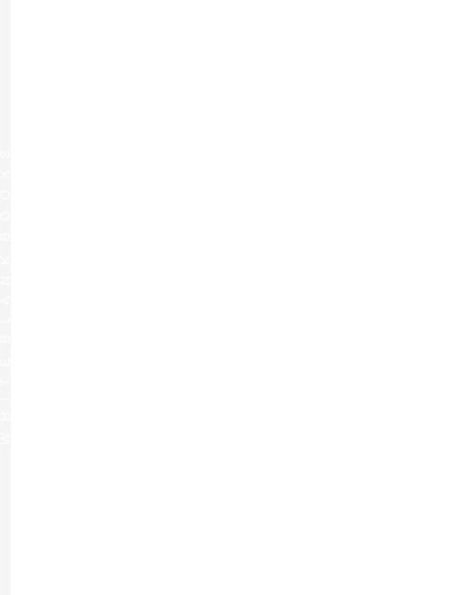
\includegraphics[height=0.2 \textheight]{Imagenes/rocas}
		\caption{Rocas cayendo cuando el jugador ha paso por el área.}
		\label{fig:rocas}
	\end{figure}